\subsection{L’importance de documenter un modèle de données}

Dans le domaine de la gestion de l'information, la documentation d’un modèle de données joue un rôle fondamental pour garantir la clarté, l'accessibilité et la pérennité des données. Une documentation bien structurée et accompagnée d'exemples contextualisés, permet non seulement de rendre les données compréhensibles, mais elle facilite également leur réutilisation et leur intégration dans divers systèmes. Cette importance est particulièrement manifeste dans les institutions culturelles et archivistiques, où la gestion de métadonnées complexes exige une documentation rigoureuse. Dans notre cas, nous avons eu besoin de traduire la documentation du modèle LIDO, déjà existante, pour donner accès à l’information en français. Mais nous ne nous sommes pas arrêtés à la traduction, nous avons adapté la documentation pour l’alimenter des divers exemples rencontrés lors de la production des mappings. \newline

\textbf{Pérennité et traçabilité des données}\newline

Un des rôles principaux de la documentation est de garantir la pérennité des données dans le temps. Les données archivistiques, par exemple, ne se limitent pas à des documents statiques, elles sont dynamiques et évoluent constamment en fonction des nouvelles acquisitions, des mises à jour ou des recherches scientifiques. C'est également vrai pour des collections de muséesn même si la description physique de l'ojbet ne va probablement pas changer, des informations sur ses origines et son histoire peuvent émerger (la recherche de provenance prends de plus d'importance dans la gestion des collections). Des données liées aux mouvements de l'objets peuvent aussi être ajoutées (sa présence dans une exposition, son déplacement vers une autre institution, etc...). \newline

Sans une documentation claire, il devient difficile de gérer les changements et d'assurer une traçabilité de l'information. Cela est particulièrement vrai pour les Archives nationales françaises, qui ont adopté des systèmes modernes comme Records in Contexts (RiC), un modèle qui permet de mieux contextualiser les données archivistiques en fonction des relations entre entités.\footcite{clavaud} \newline

En prenant l'exemple des archives, on doit noter qu'elles doivent être continuellement enrichies pour améliorer la qualité et l’exploitabilité des métadonnées. Cela nécessite de s'appuyer sur une documentation structurée qui permet de retracer l’historique des changements et des mises à jour effectuées. \newline

\textbf{Accessibilité et partage des données}\newline

Une autre raison cruciale de bien documenter un modèle de données est d'assurer l'accessibilité des informations, non seulement pour les experts techniques mais aussi pour d’autres utilisateurs comme les chercheurs ou les administrateurs. Une documentation bien rédigée agit comme une feuille de route qui guide les utilisateurs à travers les complexités des données et des relations entre elles.\newline

Par exemple, dans le contexte de la gestion des données ouvertes, la documentation devient essentielle pour permettre aux différentes parties prenantes (institutions, chercheurs, développeurs) d'accéder et de manipuler les données. Comme indiqué dans l’article de Florence Clavaud,  le partage de données entre institutions nécessite une structure de documentation solide qui facilite l’accès et garantit une utilisation correcte des informations. \footcite{clavaud}\newline, 

Au sein des Archives nationales, les chercheurs qui consultent des collections spécifiques dépendent également d’une documentation claire pour comprendre comment les archives sont structurées, classées et liées à des entités ou événements. Sans une documentation appropriée, l’accès aux informations archivées devient complexe, voire impossible. Cela peut affecter la recherche et même conduire à des erreurs dans l’interprétation des données.\newline

\textbf{Interopérabilité entre systèmes et institutions}\newline

L'interopérabilité des données entre différents systèmes et institutions repose sur la capacité à partager des informations dans des formats compatibles. Une documentation claire est essentielle pour garantir que les différents acteurs qui manipulent les données puissent utiliser des normes communes et interpréter correctement les modèles de données. Par exemple, l'intégration des métadonnées archivistiques dans des portails comme Europeana ou Archives Portal Europe nécessite l’utilisation de normes internationales comme EAD (Encoded Archival Description) et EAC-CPF (Encoded Archival Context – Corporate bodies, Persons, and Families).\newline

Le modèle LIDO-MC a vocation à structurer les flux entre les institutions et le ministère. La documentation que nous proposereons devra être officielle, validée, à la fois compréhensible au plus grand nombre dans son but, et techniquement plus complexe pour permettre des développements de connecteurs par les éditeurs logiciels de gestion des collections. \newline

\textbf{Les difficultés rencontrées lors de la documentation d’un modèle de données}\newline
Bien que la documentation d’un modèle de données soit essentielle, ce processus présente plusieurs défis qui peuvent rendre la tâche complexe.
\begin{itemize}
    \item La complexité technique des modèles
Les systèmes d'information modernes sont souvent complexes, avec des modèles de données qui incluent plusieurs entités, relations et types de données. Documenter ces modèles nécessite une compréhension approfondie de la structure des données et de leur interaction. 
    \item. Maintien de la cohérence lors de l'évolution des systèmes
Un autre défi majeur est le maintien de la cohérence entre les différentes versions d’un modèle de données à mesure que les systèmes évoluent. Parfois, les données doivent être migrées d'un système à un autre ou enrichies pour répondre à de nouveaux besoins. Cela peut entraîner des incohérences si la documentation n'est pas mise à jour correctement. 
Les Archives nationales françaises ont, par exemple, connu des difficultés lors de la mise à jour de leur système d’information archivistique (SIA) pour intégrer la plateforme d’archivage électronique ADAMANT.\footcite{clavaud} La documentation des processus et des relations entre les différentes entités était essentielle pour garantir que ces modifications n'introduisent pas d'erreurs ou de pertes d'information.
    \item La diversité des utilisateurs et des besoins
Documenter un modèle de données peut également être compliqué en raison de la diversité des utilisateurs. Alors que certains utilisateurs, comme les développeurs, ont besoin d'une documentation technique détaillée, d'autres, comme les chercheurs ou le grand public, nécessitent une documentation plus accessible et compréhensible. Trouver un équilibre entre ces différents niveaux de détail peut être difficile et demande une planification minutieuse.
Selon les principes de la gouvernance des données ouvertes, la documentation doit être 
suffisamment flexible pour répondre aux besoins des experts techniques tout en restant accessible aux non-spécialistes. Cela signifie que la documentation doit souvent être organisée en plusieurs couches, avec des détails techniques plus approfondis pour les développeurs et des explications plus simples pour les utilisateurs non techniques.

\end{itemize}

\textbf{À qui s’adresse la documentation d’un modèle de données?}\newline

La documentation d'un modèle de données s'adresse à plusieurs types d’utilisateurs, chacun ayant des besoins spécifiques en termes de détails et d'accessibilité.\newline

Les développeurs et les administrateurs de systèmes sont les principaux utilisateurs de la documentation technique. Ils ont besoin d'une compréhension détaillée de la structure des données et des relations entre les entités pour configurer, maintenir et optimiser les bases de données. Sans une documentation adéquate, ils risquent de commettre des erreurs dans la gestion des données ou de ne pas être en mesure de résoudre rapidement les problèmes qui surviennent. Ces développeurs ne sont généralement pas du personnel aux institutions, ils travaillent pour des éditeurs de logiciels. En effet, les institutions culturelles font évoluer leurs outils de plus en plus vers des outils "sur étagère" que vers des solutions développées spécifiquement. Elles préfèrent une relation commerciale classique à devoir maintenir des compétences techniques en leur sein, et devoir gérer l'obsolescence d'outils créés par strates de fonctionnalités. Donc les éditeurs sont les principaux destinataire de cette documentation.\newline

Les archivistes et chercheurs, qui utilisent les systèmes d’information pour accéder aux données archivistiques, dépendent également de la documentation. Une documentation claire leur permet de comprendre comment les données sont organisées, classées et liées entre elles. Cela leur permet non seulement d’accéder rapidement aux informations nécessaires, mais aussi de les interpréter correctement dans leurs recherches. \newline

Enfin, dans le cadre de la donnée ouverte, le grand public peut également être un utilisateur des systèmes d’information. Pour ces utilisateurs, la documentation doit être simplifiée et accessible afin de leur permettre de naviguer dans les systèmes et d'accéder aux informations sans avoir besoin d'une expertise technique avancée. Dans le domaine de la culture et des archives, l’accès du grand public aux données est souvent encouragé pour démocratiser l'information, et cela nécessite une documentation claire et concise.\newline

La documentation d’un modèle de données est une étape essentielle pour assurer la clarté, l’accessibilité et la pérennité des systèmes d’information. Elle permet de structurer les données, de garantir leur traçabilité, d’améliorer leur interopérabilité, et de faciliter leur gestion et leur partage. Cependant, ce processus présente plusieurs défis, notamment le aprocessus d’évolution des systèmes et la complexité technique des modèles. Ces défis peuvent être surmontés avec une planification rigoureuse et une mise à jour constante de la documentation. Enfin, il est essentiel que cette documentation soit adaptée aux différents publics qui l’utiliseront, qu’il s’agisse des développeurs, des chercheurs ou du grand public, afin de garantir une utilisation optimale des données et une interopérabilité entre systèmes.\newline

\textbf{Le profil d’application LIDO-MC}\newline

Un avantage du modèle LIDO est la possibilité de créer un profil d'application qui 
Un profil d’application LIDO peut contenir des éléments de restrictions, ou commander/imposer des vocabulaires spécifiques, et plus encore.
Un profil d’application est toujours un « sous-standard » de son parent. Il peut préciser la sémantique d’un élément par rapport au LIDO générique, mais il ne change jamais la sémantique de cet élément.
De plus, les éléments et attributs obligatoires ne doivent pas être déclarés facultatifs. Cela garantit qu’un enregistrement LIDO conforme à un profil d'application reste aussi conforme au standard LIDO générique.\newline

Les règles d’un profil d’application peuvent être exprimées, soit dans un document texte (html,etc…), soit par un ensemble de règles exploitables par une machine (XML Schema, Schematron).
Idéalement le profil d’application contient les 2, il fournit une documentation qui explique les règles et le contexte, et il fournit aussi un fichier exploitable par une machine qui vérifie automatiquement la conformité du document.\newline

Lors de notre stge c'est ce que nous avont choisi de faire. Pour avoir à la fois le document avec la documentation lisible par un humain, et celle avec les règles exploitable par une machine, nous avons choisi de créer un ODD (One Document Does it all).(Voir annexe).
Le LIDO Application Profile Workflow, est la manière recommandée pour créer des profils d’application. Cette méthode fournit un moyen facile de documenter les différences entre le profil d'application et le LIDO générique, ainsi que de produire de la documentation et des règles xploitables par des machines pour le profil. \newline


Le workflow se construit autour d'un fichier XML ODD définissant le profil LIDO. Ce fichier contient toutes les informations que les utilisateurs doivent fournir pour que le processus produise un profil d'application LIDO valide : les métadonnées du profil, la documentation du profil et les règles du profil. De cette manière, la définition du profil sert de source unique pour les règles exploitables par la machine ainsi que pour la documentation HTML. Chacun des fichiers de sortie est produit par une seule transformation XSL de la définition de profil.
Ces règles sont  déclarées avec des règles Schematron. La documentation du profil dans la définition du profil suit TEI-Lite et est la source principale pour la documentation HTML. \newline

\begin{figure}[h!]
	\centerline{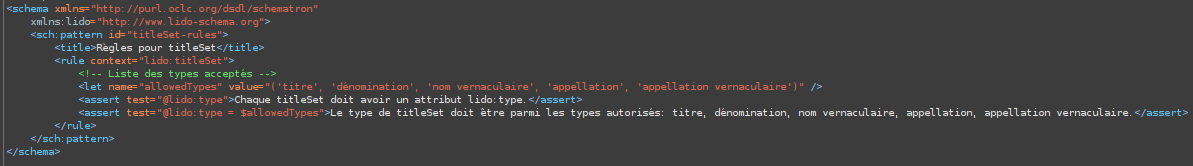
\includegraphics[width=\textwidth]{medias/exemple_schematron.png}}
	\caption{Exemple de la règle Schematron pour les TitleSet.}
\end{figure}

\begin{figure}[h!]
	\centerline{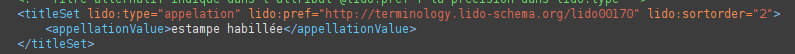
\includegraphics[width=\textwidth]{medias/exemple_attribut.png}}
	\caption{Exemple de l'usage de l'attribut autorisé.}
\end{figure}

Pour notre profil LIDO-MC, nous n'avons pas apporté de grands changemets dans les règles du LIDO générique. Ce que noous avons décidé de faire a été d'imposer une liste de termes à placer dans les attributs de certains éléments, pour qualifier des données de manière plus précise que si ont suivait les attributs propres au modèle. Ces termes peuvent notament servir à collecter des données qui ne sont pas nécessairement muséales, comme des livres, des manuscrits anciens, des films etc... Cette liste de termes a été constituée à partir des cas rencontrés lors de notre stage et est donc suceptible d'évoluer. \newline
\begin{figure}[h!]
	\centerline{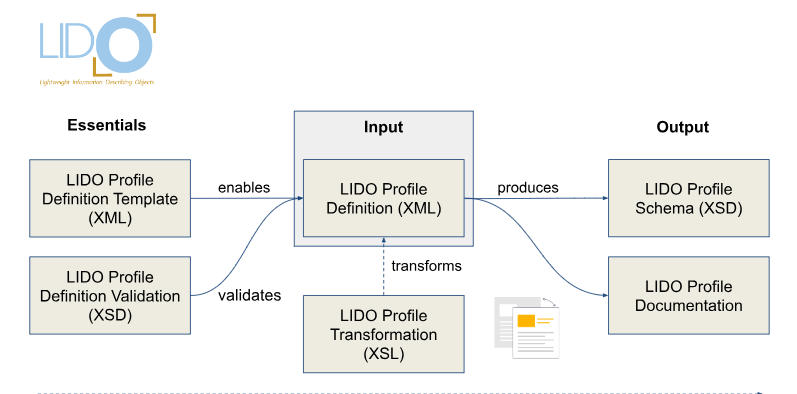
\includegraphics[width=\textwidth]{medias/Capture d’écran du 2024-09-15 07-21-40.png}}
	\caption{Workflow pour la création d'un profil d'application LIDO.\footcite{lido_primer}}
\end{figure}\newline


Notre objectif en proposant une documentation sous cette forme, est qu'elle réponde à un maximum des exigences mentionnées plus tôt, un document qui réuni toutes les informations et les règles de validation de manière structurée, devrait être suffusament adaptable pour des besoin de mis à jour. Ce document technique contient toutes les règles que les développeurs de logiciels ont besoin pour appliquer le modèle. De plus la documentation HTML produite est facilement lisible et accessible pour les autres utilisateurs. 


